%----------------------------------------------------------------------------------------
%	PACKAGES AND OTHER DOCUMENT CONFIGURATIONS
%----------------------------------------------------------------------------------------
\documentclass[11pt,a4paper,english,twoside,twocolumn]{article}
\pagenumbering{arabic}
\usepackage{setspace}
%\onehalfspace
\usepackage[hmarginratio=1:1,top=32mm,columnsep=20pt]{geometry}
\usepackage{fancyhdr}
\usepackage{multirow}
\usepackage{multicol}
\usepackage[section]{placeins}
%--Text and Style------------------------------------------------------------------------
\usepackage{microtype} 			% Slightly tweak font spacing for aesthetics
\usepackage[english]{babel} 		% Language hyphenation and typographical rules
\usepackage[T1]{fontenc}
\usepackage[utf8]{inputenc}
\usepackage{ae}
\usepackage{relsize}
\usepackage{csquotes} 
\usepackage{amsmath}
\usepackage{amsfonts}
\usepackage{mathdots}
\usepackage{mathtools}
\usepackage[colorlinks=true]{hyperref}
\hypersetup{
	bookmarksnumbered=true,
	linkcolor=black,
	citecolor=black,
	%pagecolor=black,
	urlcolor=black,
}
\usepackage{verbatim}
\usepackage{alltt}
\DeclareMathOperator{\sgn}{sgn}
\DeclareMathOperator{\RealNumber}{\rm I\!R}
\DeclarePairedDelimiter{\abs}{\lvert}{\rvert}
\DeclarePairedDelimiter{\norma}{\lVert}{\rVert}

%---Figure------------------------------------------------------------------------------

\usepackage{graphicx}
\graphicspath{{./imgs/}}
\renewcommand{\figurename}{Fig.}
\usepackage{subfig}

%---------------------------------------------------------------------------------------
\usepackage{algorithmicx}
\usepackage[ruled]{algorithm}
\usepackage{algpseudocode}
\usepackage{listings}
\usepackage{xcolor}
\definecolor{maroon}{cmyk}{0, 0.87, 0.68, 0.32}
\definecolor{halfgray}{gray}{0.55}
\definecolor{ipython_frame}{RGB}{207, 207, 207}
\definecolor{ipython_bg}{RGB}{247, 247, 247}
\definecolor{ipython_red}{RGB}{186, 33, 33}
\definecolor{ipython_green}{RGB}{0, 128, 0}
\definecolor{ipython_cyan}{RGB}{64, 128, 128}
\definecolor{ipython_purple}{RGB}{170, 34, 255}
\lstset{
    breaklines=true,
    %
    extendedchars=true,
    literate=
    {á}{{\'a}}1 {é}{{\'e}}1 {í}{{\'i}}1 {ó}{{\'o}}1 {ú}{{\'u}}1
    {Á}{{\'A}}1 {É}{{\'E}}1 {Í}{{\'I}}1 {Ó}{{\'O}}1 {Ú}{{\'U}}1
    {à}{{\`a}}1 {è}{{\`e}}1 {ì}{{\`i}}1 {ò}{{\`o}}1 {ù}{{\`u}}1
    {À}{{\`A}}1 {È}{{\'E}}1 {Ì}{{\`I}}1 {Ò}{{\`O}}1 {Ù}{{\`U}}1
    {ä}{{\"a}}1 {ë}{{\"e}}1 {ï}{{\"i}}1 {ö}{{\"o}}1 {ü}{{\"u}}1
    {Ä}{{\"A}}1 {Ë}{{\"E}}1 {Ï}{{\"I}}1 {Ö}{{\"O}}1 {Ü}{{\"U}}1
    {â}{{\^a}}1 {ê}{{\^e}}1 {î}{{\^i}}1 {ô}{{\^o}}1 {û}{{\^u}}1
    {Â}{{\^A}}1 {Ê}{{\^E}}1 {Î}{{\^I}}1 {Ô}{{\^O}}1 {Û}{{\^U}}1
    {œ}{{\oe}}1 {Œ}{{\OE}}1 {æ}{{\ae}}1 {Æ}{{\AE}}1 {ß}{{\ss}}1
    {ç}{{\c c}}1 {Ç}{{\c C}}1 {ø}{{\o}}1 {å}{{\r a}}1 {Å}{{\r A}}1
    {€}{{\EUR}}1 {£}{{\pounds}}1
}

%%
%% Python definition (c) 1998 Michael Weber
%% Additional definitions (2013) Alexis Dimitriadis
%% modified by me (should not have empty lines)
%%
\lstdefinelanguage{iPython}{
    morekeywords={access,and,break,class,continue,def,del,elif,else,except,exec,finally,for,from,global,if,import,in,is,lambda,not,or,pass,print,raise,return,try,while},%
    %
    % Built-ins
    morekeywords=[2]{abs,all,any,basestring,bin,bool,bytearray,callable,chr,classmethod,cmp,compile,complex,delattr,dict,dir,divmod,enumerate,eval,execfile,file,filter,float,format,frozenset,getattr,globals,hasattr,hash,help,hex,id,input,int,isinstance,issubclass,iter,len,list,locals,long,map,max,memoryview,min,next,object,oct,open,ord,pow,property,range,raw_input,reduce,reload,repr,reversed,round,set,setattr,slice,sorted,staticmethod,str,sum,super,tuple,type,unichr,unicode,vars,xrange,zip,apply,buffer,coerce,intern},%
    %
    sensitive=true,%
    morecomment=[l]\#,%
    morestring=[b]',%
    morestring=[b]",%
    %
    morestring=[s]{'''}{'''},% used for documentation text (mulitiline strings)
    morestring=[s]{"""}{"""},% added by Philipp Matthias Hahn
    %
    morestring=[s]{r'}{'},% `raw' strings
    morestring=[s]{r"}{"},%
    morestring=[s]{r'''}{'''},%
    morestring=[s]{r"""}{"""},%
    morestring=[s]{u'}{'},% unicode strings
    morestring=[s]{u"}{"},%
    morestring=[s]{u'''}{'''},%
    morestring=[s]{u"""}{"""},%
    %
    % {replace}{replacement}{lenght of replace}
    % *{-}{-}{1} will not replace in comments and so on
    literate=
    {á}{{\'a}}1 {é}{{\'e}}1 {í}{{\'i}}1 {ó}{{\'o}}1 {ú}{{\'u}}1
    {Á}{{\'A}}1 {É}{{\'E}}1 {Í}{{\'I}}1 {Ó}{{\'O}}1 {Ú}{{\'U}}1
    {à}{{\`a}}1 {è}{{\`e}}1 {ì}{{\`i}}1 {ò}{{\`o}}1 {ù}{{\`u}}1
    {À}{{\`A}}1 {È}{{\'E}}1 {Ì}{{\`I}}1 {Ò}{{\`O}}1 {Ù}{{\`U}}1
    {ä}{{\"a}}1 {ë}{{\"e}}1 {ï}{{\"i}}1 {ö}{{\"o}}1 {ü}{{\"u}}1
    {Ä}{{\"A}}1 {Ë}{{\"E}}1 {Ï}{{\"I}}1 {Ö}{{\"O}}1 {Ü}{{\"U}}1
    {â}{{\^a}}1 {ê}{{\^e}}1 {î}{{\^i}}1 {ô}{{\^o}}1 {û}{{\^u}}1
    {Â}{{\^A}}1 {Ê}{{\^E}}1 {Î}{{\^I}}1 {Ô}{{\^O}}1 {Û}{{\^U}}1
    {œ}{{\oe}}1 {Œ}{{\OE}}1 {æ}{{\ae}}1 {Æ}{{\AE}}1 {ß}{{\ss}}1
    {ç}{{\c c}}1 {Ç}{{\c C}}1 {ø}{{\o}}1 {å}{{\r a}}1 {Å}{{\r A}}1
    {€}{{\EUR}}1 {£}{{\pounds}}1
    %
    {^}{{{\color{ipython_purple}\^{}}}}1
    {=}{{{\color{ipython_purple}=}}}1
    %
    {+}{{{\color{ipython_purple}+}}}1
    {*}{{{\color{ipython_purple}$^\ast$}}}1
    {/}{{{\color{ipython_purple}/}}}1
    %
    {+=}{{{+=}}}1
    {-=}{{{-=}}}1
    {*=}{{{$^\ast$=}}}1
    {/=}{{{/=}}}1,
    literate=
    *{-}{{{\color{ipython_purple}-}}}1
     {?}{{{\color{ipython_purple}?}}}1,
    %
    identifierstyle=\color{black}\ttfamily,
    commentstyle=\color{ipython_cyan}\ttfamily,
    stringstyle=\color{ipython_red}\ttfamily,
    keepspaces=true,
    showspaces=false,
    showstringspaces=false,
    %
    rulecolor=\color{ipython_frame},
    frame=single,
    frameround={t}{t}{t}{t},
    framexleftmargin=6mm,
    numbers=left,
    numberstyle=\tiny\color{halfgray},
    %
    %
    backgroundcolor=\color{ipython_bg},
    %   extendedchars=true,
    basicstyle=\scriptsize,
    keywordstyle=\color{ipython_green}\ttfamily,
}

%------for matlab scheme color-code----------------------------------
\definecolor{mygreen}{RGB}{28,172,0} % color values Red, Green, Blue
\definecolor{mylilas}{RGB}{170,55,241}
\lstset{language=Matlab,%
    %basicstyle=\color{red},
    breaklines=true,%
    morekeywords={matlab2tikz},
    keywordstyle=\color{blue},%
    morekeywords=[2]{1}, keywordstyle=[2]{\color{black}},
    identifierstyle=\color{black},%
    stringstyle=\color{mylilas},
    commentstyle=\color{mygreen},%
    %without this there will be a symbol in the places where there is a space
    showstringspaces=false,
    numbers=left,%
    % size of the numbers
    numberstyle={\tiny \color{black}},
    numbersep=9pt, % this defines how far the numbers are from the text
    emph=[1]{for,end,break},emphstyle=[1]\color{blue}, %some words to emphasise
    emph=[2]{cos,sin,length, pi}, emphstyle=[2]\color{black},
    %
    %rulecolor=\color{ipython_frame},
    frame=single,
    frameround={t}{t}{t}{t},
    framexleftmargin=6mm,
    numbers=left,
    numberstyle=\tiny\color{halfgray},
    %
    %
    backgroundcolor=\color{ipython_bg},
    basicstyle=\scriptsize,   
}

%----Table------------------------------------------------------------------------------
\usepackage{tabularx}
\usepackage{array}
\usepackage{color}
\usepackage{adjustbox}
\usepackage{colortbl}
\usepackage{pgfplotstable}
\usepackage{makecell}
\usepackage{booktabs}

%----------------------------------------------------------------------------------------
% Allows abstract customization
\usepackage{abstract}

% Set the "Abstract" text to bold
\renewcommand{\abstractnamefont}{\normalfont\bfseries} 
% Set the abstract itself to small italic text
\renewcommand{\abstracttextfont}{\normalfont\small\itshape} 

% Allows customization of titles
\usepackage{titlesec} 

% Roman numerals for the sections
\renewcommand\thesection{\Roman{section}} 

% roman numerals for subsections
\renewcommand\thesubsection{\roman{subsection}} 

% Change the look of the section titles
\titleformat{\section}[block]{\large\scshape\centering}{\thesection.}{1em}{} 

% Change the look of the section titles
\titleformat{\subsection}[block]{\large}{\thesubsection.}{1em}{} 
\usepackage{titling} % Customizing the title section

%----------------------------------------------------------------------------------------
\usepackage{tikz,fp,ifthen,fullpage}
\usepackage{pgfmath, pgfplots, xparse}
\usetikzlibrary{backgrounds, arrows}
\usetikzlibrary{decorations.pathmorphing,fit,through}
\usetikzlibrary{shapes,decorations,shadows}
\usetikzlibrary{fadings,patterns,mindmap}
\usepackage{tikz-dimline, calc}
\pgfplotsset{compat=newest}

%----------------------------------------------------------------------------------------
%	TITLE SECTION
%----------------------------------------------------------------------------------------
\setlength{\droptitle}{-4\baselineskip} % Move the title up


\pretitle{\begin{center}\Huge\bfseries} % Article title formatting


\posttitle{\end{center}} % Article title closing formatting


\title{Homework - Kinematics Calibration of a Differential drive wheelchair} % Article title

\author{%
	% Your name
	\textsc{Francesco Argentieri}\thanks{ID: 183892}\\[1ex] 
	% Your institution
	\normalsize University of Trento \\ 
	% Your email address
	\normalsize \href{mailto:francesco.argentieri@studenti.unitn.it}{francesco.argentieri@studenti.unitn.it} 
}
%\and % Uncomment if 2 authors are required, duplicate these 4 lines if more
%\textsc{Jane Smith}\thanks{Corresponding author} \\[1ex] % Second author's name
%\normalsize University of Utah \\ % Second author's institution
%\normalsize \href{mailto:jane@smith.com}{jane@smith.com} % Second author's email address

% Leave empty to omit a date
\date{} 
\renewcommand{\maketitlehookd}{%
	\begin{abstract}
		\noindent  For a mobile robot, odometry calibration consists of the identification of a set of kinematic parameters that allow reconstructing the vehicle’s relative position and orientation starting from the wheels’ encoder measurements.
The aim of the homework is to:
estimate from the encoder and the camera data the kinematics parameters wheels radius “$r_\textsc{l}$" and “$r_\textsc{r}$" and wheelbase “b".
Estimate the camera position with respect to the wheelchair reference point (the mid point between the wheels).
\end{abstract}
}

%----------------------------------------------------------------------------------------
\begin{document}
	% Print the title
	\maketitle
	
	%Other chapter
	\section{Introduction}
The autonomous navigation is understood as the set of techniques by which it is a system able to move with a certain level of autonomy in a certain type of environment (land, air, underwater, space). The problems in the field of autonomous navigation are addressed first and foremost related to the localization of the system with respect to the environment, planning out their duties and motion control.
An interesting class of systems covered by the study of autonomous navigation systems is that of the AGV (Autonomous Guided Vehicles). They are now widely used in industries, ports, airports, hospitals, etc, however, to measure the position and the attitude of a vehicle it is still a problem of substantial interest.
The sensor fusion is the process that combines information from a number of different sources to provide a complete and robust description (measure) a set of variables of interest. The sensor fusion is of particular utility in any application where many measures have to be combined together, melted and optimized in order to obtain quality information and integrity suitable for the purpose of the application. The sensor fusion techniques are used in many industrial systems, military, monitoring, civilian surveillance, control processes and systems. The problem of localization of autonomous vehicles, which in almost all cases, the individual transducers are found insufficient in setting up a comprehensive and robust localization system for autonomous navigation, requires the use of sensor fusion techniques for combining measurements from different types of transducers whose characteristics, if fused together, allow us to obtain a more reliable and accurate measure of the state of the system and the environment surrounding it.
The sensor fusion techniques have important applications in the field of autonomous navigation, in which it is necessary to obtain a good estimate of the position measurement and alignment (pose) of a mobile robot. Incremental measuring methods or dead-reckoning, using encoders, gyroscopes utrasuoni etc., have the considerable advantages of being self-contained within the robot, to be relatively simple to use and provide high refresh rate measure. On the other hand, since these measurement systems integrate related increments, the errors grow considerably increasing the integration time.
The document presented is based on the analysis of a real robot, developed and built at the MIRO - Measurements Instrumentations Robotics Lab at the University of Trento.
It is equipped with two rotary incremental encoder keyed to the axes of the two wheels and a chamber pointing upwards for reading specially arranged on the ceiling marker.
The two datasets have been collected steering the vehicle clockwise and counterclockwise.
The aim of the homework is to:
\begin{itemize}
\item Estimate from the encoder and the camera data the kinematics parameters wheels radius Rl and Rr and wheelbase b.
\item Estimate the camera position with respect to the wheelchair reference point (the mid point between the wheels).
\end{itemize}
	\section{Methods}
\subsection{Kinematic Model}
For the analysis of differential wheelchair drive parameters using a simplified model in the reference system own odometric placed in the center of the robot indicated by $RF1$. Consider that moves in a reference system fixed to the $RF0$ envoiroment. The robot is subject to pure rolling, then we neglect slippage between wheel and ground. The angular velocities, indicated respectively with omega, are applied respectively to the right and left wheels in such a way that the components of the fixed body and the speed of the robot are related to the angu- lar velocity of the wheels according to the equation functional \ref{eq:velocityrelation}. The other two support wheels are considered passive. This schematization is observable in fig. \ref{fig:model}.
\begin{equation}
\label{eq:velocityrelation}
	\left[ \begin{array}{cc}
				v	\\									
				\omega 							
			 \end{array} 
	\right]  =\, C\,
	\left[ \begin{array}{cc}
 				\omega_\textsc{l} \\ 
				\omega_\textsc{r}
			 \end{array} 
	\right]
\end{equation}

\begin{figure}[!h]
\centering
    \resizebox{.8\linewidth}{!}{\begin{tikzpicture} [>=latex]
% \draw [help lines] (0,0) grid (8, 8);
% \foreach \x in {0,1,...,8}
%   \draw [help lines] (\x,0) node [below,%
%          font=\footnotesize] {$\x$} -- (\x,0);
%\foreach \y in {0,1,...,8}
%   \draw [help lines] (0,\y) node [left,%
%          font=\footnotesize] {$\y$} -- (0,\y);
 % body robot
 \draw [fill=lightgray, fill opacity=0.5](4, 4) circle (2.25);
 \draw [rounded corners=15,pattern=crosshatch, pattern color=gray] (0.5, 2.5)  rectangle (1.5, 5.5);
 \draw [rounded corners=15,pattern=crosshatch, pattern color=gray] (6.5, 2.5) rectangle (7.5, 5.5);
 \draw (1.5, 4) -- (6.5, 4);
 % quote wheel
 \dimline  [color=gray, 
                 %line style={thick},
                %extension start style={gray,thin},
                %extension end style={gray,thin},
               extension start length=1cm,
              extension end length=1cm,
                ]{(0, 4)}{ (0, 5.5)}{$r$};
 % quote track
 \dimline    [color=gray,
                % line style={thick},
                %extension start style={gray,thin},
                %extension end style={gray,thin},
                extension start length=-1cm,
                extension end length=-1cm
                ]{(1, 1.25)}{ (7, 1.25)}{$b$};
 % vector
 	\draw [->, blue] (4, 6) -- (4, 8) node[left]{$v$};
 	\draw [->, red] (1, 4) -- (1,7) node[left]{$\omega_{r}$};
 	\draw [->, red] (7, 4) -- (7,7)	 node[left]{$\omega_{l}$};
	\draw [->, orange] (4.75,4) arc (0:(-300+45):0.75) node[below]{$\omega$};
 % Reference system 0
 	\coordinate [label = below: \scriptsize $RF0$] (A) at (0,0);
 	\coordinate	(Bx) at	($(A)+1*(0:1)$);
 	\coordinate	(By)	at	($(A)+1*(90:1)$);
 	\draw [->] 	(A) -- (By) node[left]{$y$};
 	\draw [->] 	(A) -- (Bx) node[above]{$x$};
 % RF1
  	\coordinate [label = below: \scriptsize $RF1$] (RF1) at (4,4);
 	\coordinate	(RF1x) at	($(RF1)+1*(0:1)$);
 	\coordinate	(RF1y)	at	($(RF1)+1*(90:1)$);
 	\fill(RF1) circle (1.4pt);
 	\draw [->] (RF1) -- (RF1y) node[left] {$y'$};
 	\draw [->] (RF1) -- (RF1x) node[above] {$x'$};
 % RFcam
 	\coordinate [label = below: \scriptsize $RF_{cam}$] (R) at (4.3,2.8);
 	\coordinate (Rx) at ($(R)+1*(22.5:1)$);
 	\coordinate (Ry) at ($(R)+1*(90+22.5:1)$);
 	\fill (R) circle (1.4pt);
	 \draw [->, darkgray] (R) -- (Ry) node[left] {$y_{cam}$};
 	 \draw [->, darkgray] (R) -- (Rx) node[above]{$x_{cam}$};
 \end{tikzpicture}}
\caption{Robot kinematic model}
\label{fig:model}
\end{figure}
\noindent Where the matrix $\textbf{C} \in \RealNumber^{2 x 2}$ is defined as (\ref{eq:Cmatrix}):
\begin{equation}
\label{eq:Cmatrix}
	\left[ \begin{array}{cc}
 				\frac{r_\textsc{r}}{2} &	\frac{r_\textsc{l}}{2} \\
				\frac{r_\textsc{l}}{b} &	-\frac{r_\textsc{l}}{b} 
			 \end{array} 
	\right]
\end{equation}
in which $r_\textsc{r}$ and $r_\textsc{l}$ are the radii of the right and left wheel, respectively.
The odometry of a vehicle is usually implemented by discrete-time integration, such as (\ref{eq:odometry}):
\begin{equation}
\label{eq:odometry}
	\begin{cases}
		x_{k+1} = x_{k} + T \, v_{k} \, cos(\theta_{k} + T \,\omega_{k}/2)\\
		y_{k+1} = y_{k} + T \, v_{k} \, sin(\theta_{k} + T \, \omega_{k}/2)\\
		\theta_{k+1} = \theta_{k} + T \, \omega_{k}
	\end{cases}
\end{equation}
Notice that low sampling frequency and high vehicle velocities can be a significant source of odometric error.
\subsection{Data Analysis}
To achieve the objective of calibration of the geometric parameters of the robot there were provided four datasets where in each of which collected the information from the camera and from the incremental encoder.
First data operation was carried out by a python script to correct the angle sign registered as evaluated with a negative sign.
Second operation and change the left encoder incremental measuring as being mounted on reverse respect to the right its value must be taken with a negative sign.
In the file is observed the possibility of the presence of two successive rows with the same timestamp. This means that at the same time have been changed both the encoder ticks and the camera pose or covariance.
It may be noted that in one line has changed the camera information and the other the odometer ticks. Thus, at the same timestamp, in the second row is the information are modified.
So you chose to eliminate duplicate rows preserve the last where both information camera pose or covariance and ticks has changed.
To achieve this, it is made use of the possibilities offered by data structures provided by Python fact realizing a dictionary between camera pose values and covariance, so it was possible to compare multiple values at the same instant and eliminate redundant data.
\subsection{Calibration Techinque}
To estimate the parameters of the robot expressed in the equation \ref{eq:Cmatrix}, namely, the wheel radius values indicated with ``$r_\textsc{r}$" and ``$r_\textsc{l}$", and the axle track as indicated ``$b$", using the method described in the report \cite{1512356}.
Experiments of odometry calibration require measurement of the absolute position and orientation of the mobile robot at suitable locations along the motion trajectories. For instance this calibration technique requires measurement of the starting and final robot configuration for each motion execution. The datasets supplied information related to: the camera position $x, y, \theta$ and increments of the encoder.
Each information is saved in columns:
\begin{itemize}
\item column 1: acquisistions time [ms];
\item columns 2--3--4: camera pose $x, y, \theta$ [cm, cm, rad];
\item column from 5 to 13: camera covariance ordered by rows [cm$2^2$] for pose, [rad$^2$] for angle and [cm*rad] for mixed terms;
\item colunm 14--15: odometric Encoder ticks Left and Right;
\end{itemize}
It has been chosen to perform the odometry calibration whereas in the same calculation all four datasets provided as suggested by the technique used. Then the equations (\ref{eq:Phi4}) and (\ref{eq:XY4}) are rewritten limited to the four paths to obtain:
\begin{equation}
\label{eq:Phi4}
	\begin{bmatrix}
		\hat{c}_{2,1}\\
		\hat{c}_{2,2}
	\end{bmatrix} =	(\bar{\Phi}_{\theta}^{\textsc{t}} \, \bar{\Phi}_{\theta})^{-1} \, \bar{\Phi}_{\theta}^{\textsc{t}} \, 
	\begin{bmatrix}
		\theta_{\textsc{n},1} - \theta_{\textsc{n},0}\\
		\theta_{\textsc{n},2} - \theta_{\textsc{n},0}\\
		\theta_{\textsc{n},3} - \theta_{\textsc{n},0}\\
		\theta_{\textsc{n},4} - \theta_{\textsc{n},0}
	\end{bmatrix}
\end{equation}
\begin{equation}
\label{eq:XY4}
	\begin{bmatrix}
		\hat{c}_{1,1}\\
		\hat{c}_{1,2}
	\end{bmatrix} = (\bar{\Phi}_{xy}^{\textsc{t}} \, \bar{\Phi}_{xy})^{-1} \, \bar{\Phi}_{xy}^{\textsc{t}} \, 
	\begin{bmatrix}
		xy_{\textsc{n},1} - xy_{\textsc{n},0}\\
		xy_{\textsc{n},2} - xy_{\textsc{n},0}\\
		xy_{\textsc{n},3} - xy_{\textsc{n},0}\\
		xy_{\textsc{n},4} - xy_{\textsc{n},0}
	\end{bmatrix}
\end{equation}
 As a result of simulations shows the values of the matrix C:
\begin{equation}
\label{eq:Cresult}
	\begin{bmatrix}
		8.1873  &  6.5229\\
    	0.2823 &  -0.2807
	\end{bmatrix}
\end{equation}
It is noted that the parameters $c_{1,1}$ and $c_{1,2}$ relative to the spokes of the wheels are different from each other, this is due to the simplifications introduced by the kinematic model. On the other hands, the axle values, $c_ {2,1}$ and $c_ {2,2}$, without the negative sign, are much more similar because formerly esti- mated at $c_{1,j}$ therefore do not contain the error propagation. Subsequently, it calcu- lates the average between the values of the obtained rays and the standard deviation, these are shown in table (\ref{tab:recapvalue}).
\begin{table}[!h]
\centering
	\begin{tabular}{lccc}
		\hline
								& Radius 	& Mean 	& standard\\
								&	[mm]	& [mm]	& deviation [mm]\\
		\hline
		$r_\textsc{r}$	&	$130.457$		& $147.102	$		&	$\pm23.538$\\
		$r_\textsc{l}$	&	$163.746$		& $147.102	$		&	$\pm23.538$\\
		$b$					&	$522.43$\\
		\hline
\end{tabular}
\caption{estimated value}
\label{tab:recapvalue}
\end{table}
\\Finally, we show in figures \ref{fig:OdoRec}, it shows the calculation for each path odometric with parameters previously estimated in comparison with the trajectory recorded by the camera.
\begin{figure*}[htb]
\centering
\subfloat[][\emph{dataset 1}.]
   {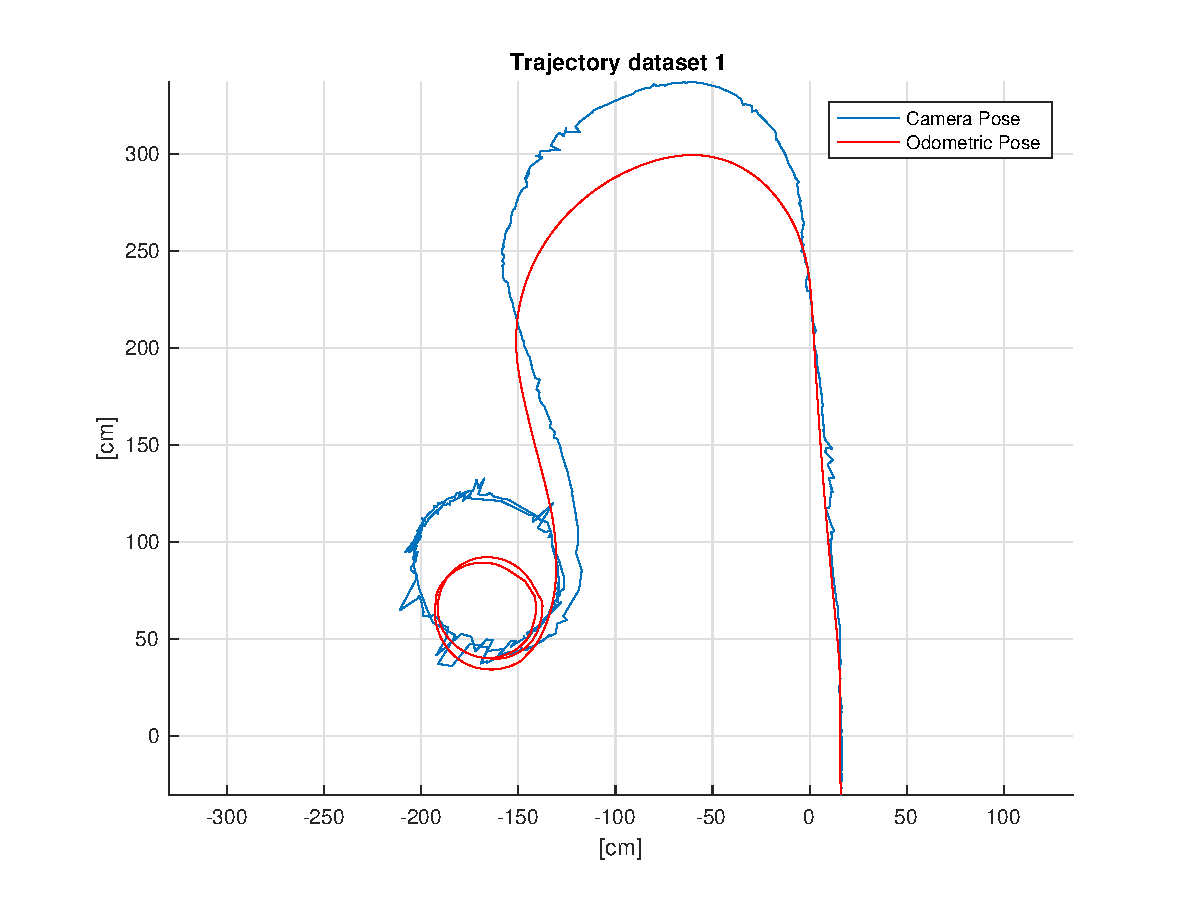
\includegraphics[width=0.45\textwidth]{odometric_1.eps}} \,
\subfloat[][\emph{dataset 2}.]
   {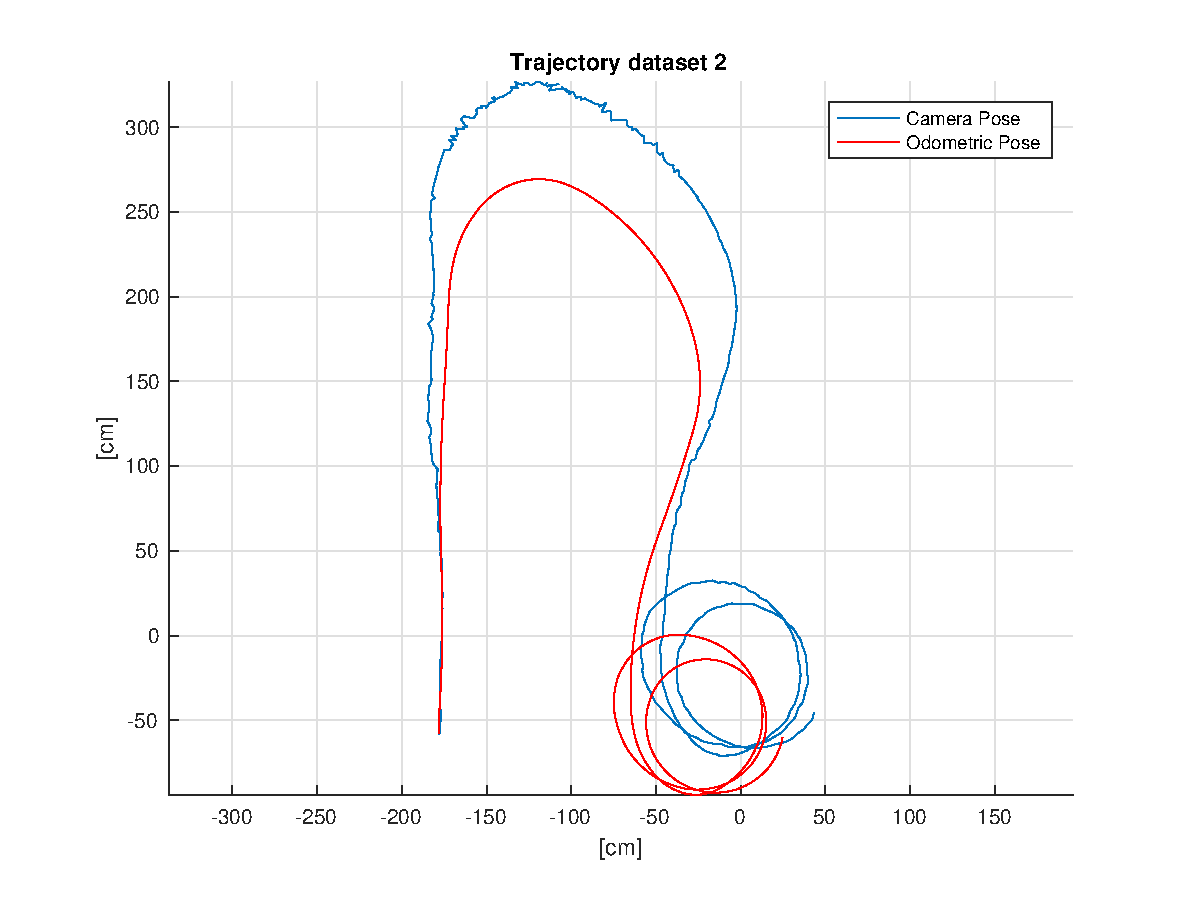
\includegraphics[width=0.45\textwidth]{odometric_2.eps}} \\
\subfloat[][\emph{dataset 3}.]
   {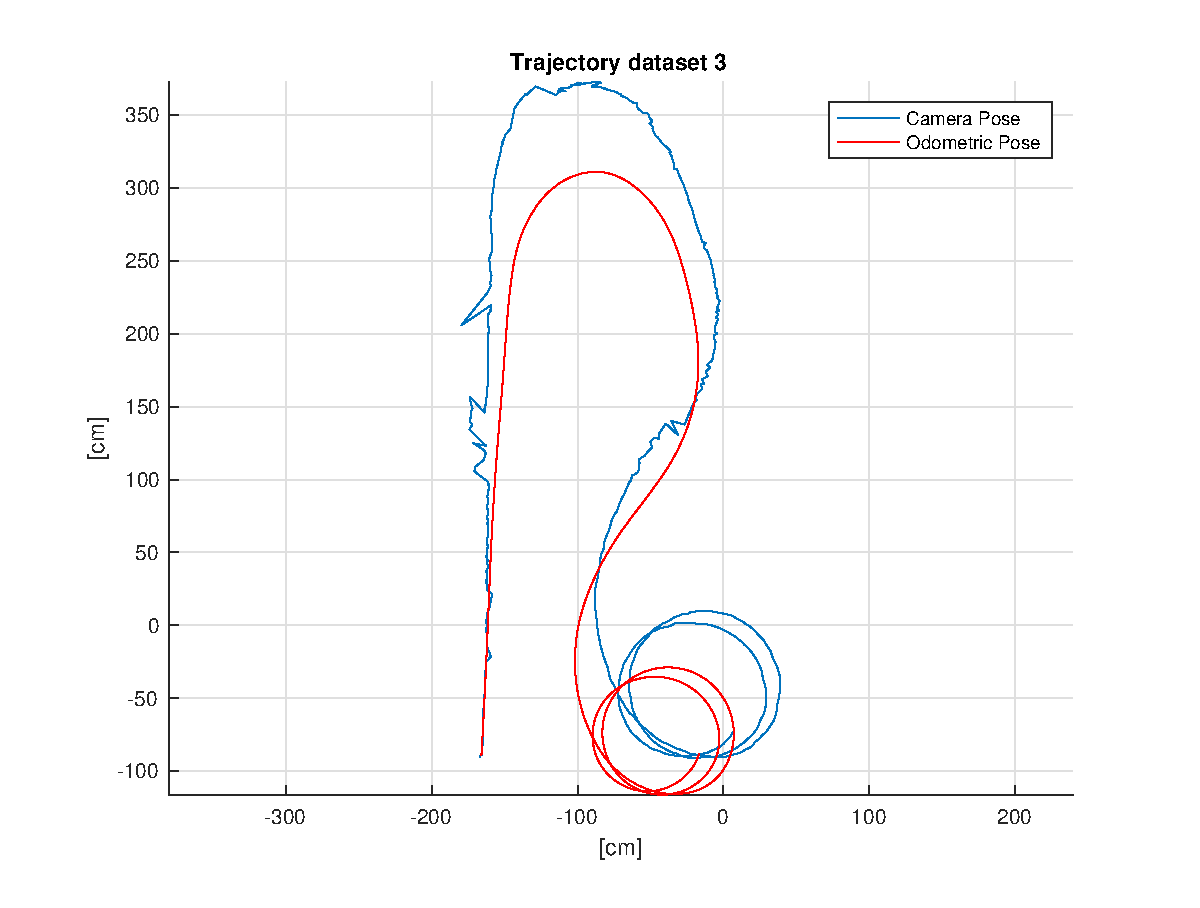
\includegraphics[width=0.45\textwidth]{odometric_3.eps}} \,
\subfloat[][\emph{dataset 4}.]
   {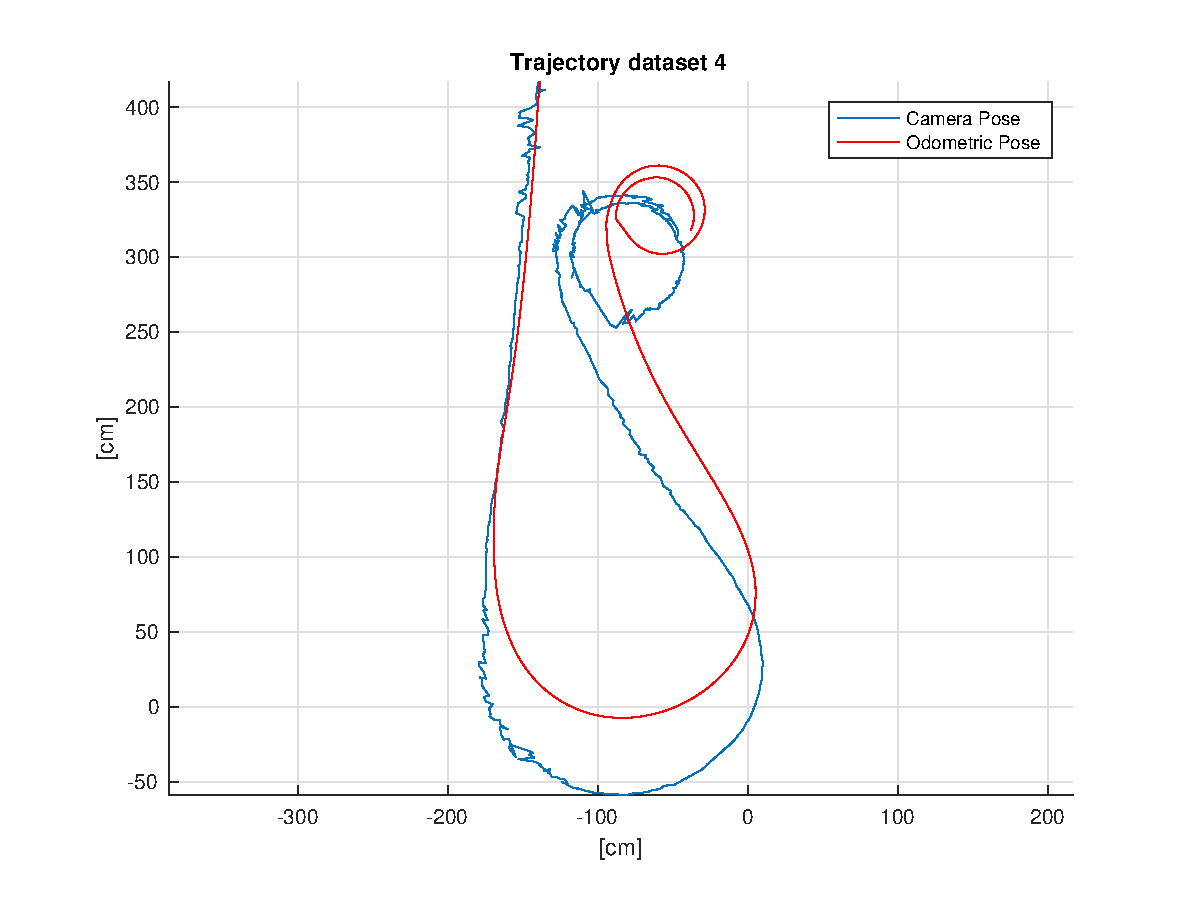
\includegraphics[width=0.45\textwidth]{odometric_4.eps}}
\caption{Odometry reconstruction}
\label{fig:OdoRec}
\end{figure*}

\subsection{Optimization}
\begin{figure*}[htb]
\centering
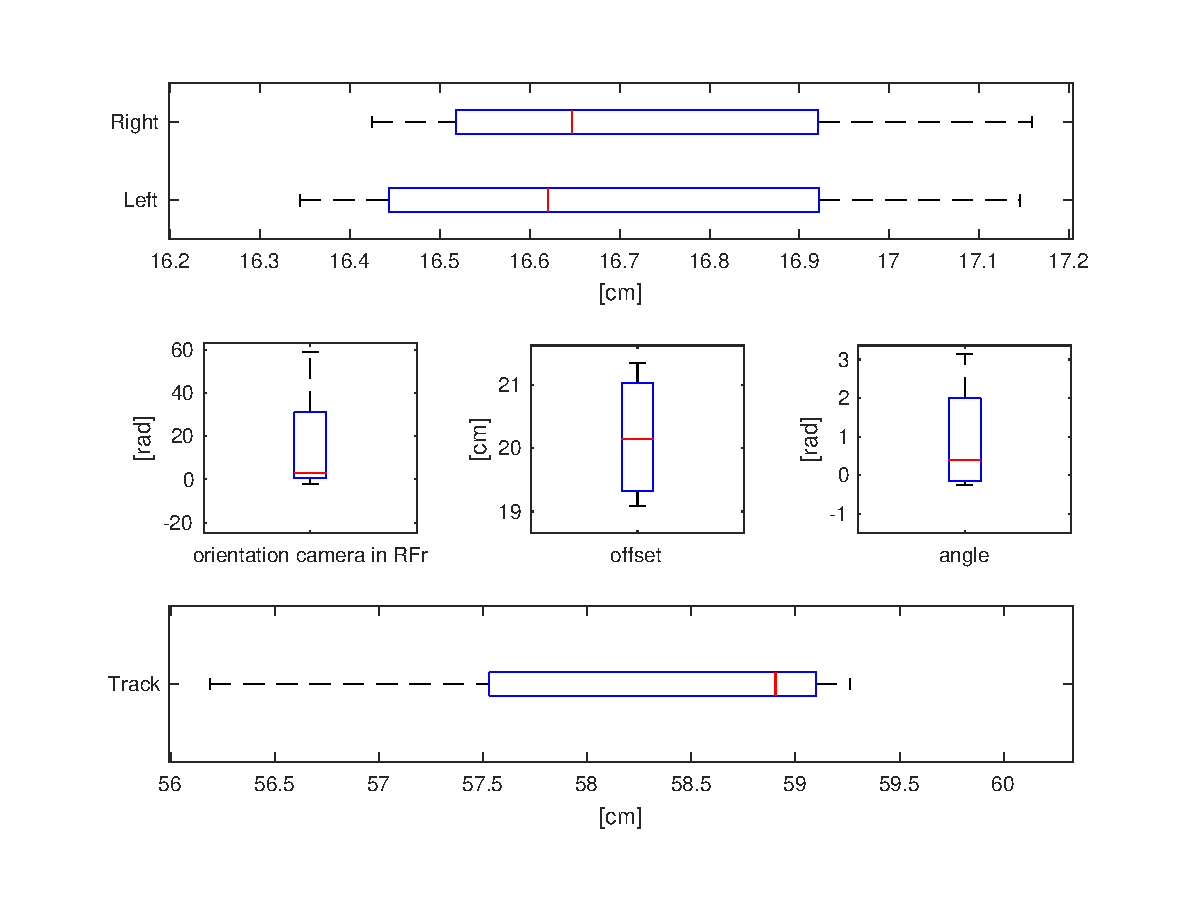
\includegraphics[width=.9\textwidth]{boxplot}
\caption{optimization among all dataset}
\label{fig:boxplot}
\end{figure*}
To achieve the goal of determining the offset of the camera mounted on the robot, it is resorted to multivariable optimization. oppurtanamente choices using six variables. Using the parameters obtained previously, summarized in the table \ref{tab:recapvalue}, they were used as the boundary conditions limits.
The algorithm used is part of the family of ``\emph{genetic algorithms} \cite{wiki:xxx}'' used for finding optimal solution.
In a genetic algorithm, a population of candidate solutions (called individuals, creatures, or phenotypes) to an optimization problem is evolved toward better solutions. Each candidate solution has a set of properties which can be mutated and altered; traditionally, solutions are represented in binary as strings of $0s$ and $1s$, but other encodings are also possible \cite{Whitley1994}.
The evolution usually starts from a population of randomly generated individuals, and is an iterative process, with the population in each iteration called a generation. In each generation, the fitness of every individual in the population is evaluated; the fitness is usually the value of the objective function in the optimization problem being solved. The more fit individuals are stochastically selected from the current population, and each individual's genome is modified (recombined and possibly randomly mutated) to form a new generation. The new generation of candidate solutions is then used in the next iteration of the algorithm. Commonly, the algorithm terminates when either a maximum number of generations has been produced, or a satisfactory fitness level has been reached for the population.
A typical genetic algorithm requires:
\begin{itemize}
\item a genetic representation of the solution domain,
\item a fitness function to evaluate the solution domain.
\end{itemize}
A standard representation of each candidate solution is as an array of bits\cite{Whitley1994}. Arrays of other types and structures can be used in essentially the same way. The main property that makes these genetic representations convenient is that their parts are easily aligned due to their fixed size, which facilitates simple crossover operations. Variable length representations may also be used, but crossover implementation is more complex in this case. Tree-like representations are explored in genetic programming and graph-form representations are explored in evolutionary programming; a mix of both linear chromosomes and trees is explored in gene expression programming.
Once the genetic representation and the fitness function are defined, a GA proceeds to initialize a population of solutions and then to improve it through repetitive application of the mutation, crossover, inversion and selection operators.
The population size depends on the nature of the problem, but typically contains several hundreds or thousands of possible solutions. Often, the initial population is generated randomly, allowing the entire range of possible solutions (the search space). Occasionally, the solutions may be ``seeded" in areas where optimal solutions are likely to be found.
During each successive generation, a portion of the existing population is selected to breed a new generation. Individual solutions are selected through a fitness-based process, where fitter solutions (as measured by a fitness function) are typically more likely to be selected. Certain selection methods rate the fitness of each solution and preferentially select the best solutions. Other methods rate only a random sample of the population, as the former process may be very time-consuming.
The fitness function is defined over the genetic representation and measures the quality of the represented solution. The fitness function is always problem dependent. For instance, in the knapsack problem one wants to maximize the total value of objects that can be put in a knapsack of some fixed capacity. A representation of a solution might be an array of bits, where each bit represents a different object, and the value of the bit (0 or 1) represents whether or not the object is in the knapsack. Not every such representation is valid, as the size of objects may exceed the capacity of the knapsack. The fitness of the solution is the sum of values of all objects in the knapsack if the representation is valid, or $0$ otherwise.
In some problems, it is hard or even impossible to define the fitness expression; in these cases, a simulation may be used to determine the fitness function value of a phenotype, or even interactive genetic algorithms are used.
The next step is to generate a second generation population of solutions from those selected through a combination of genetic operators: crossover, and mutation.
For each new solution to be produced, a pair of ``parent" solutions is selected for breeding from the pool selected previously. By producing a "child" solution using the above methods of crossover and mutation, a new solution is created which typically shares many of the characteristics of its ``parents". New parents are selected for each new child, and the process continues until a new population of solutions of appropriate size is generated. Although reproduction methods that are based on the use of two parents are more ``biology inspired", some research suggests that more than two ``parents" generate higher quality chromosomes.
These processes ultimately result in the next generation population of chromosomes that is different from the initial generation. Generally the average fitness will have increased by this procedure for the population, since only the best organisms from the first generation are selected for breeding, along with a small proportion of less fit solutions. These less fit solutions ensure genetic diversity within the genetic pool of the parents and therefore ensure the genetic diversity of the subsequent generation of children.
Although crossover and mutation are known as the main genetic operators, it is possible to use other operators such as regrouping, colonization-extinction, or migration in genetic algorithms.
It is worth tuning parameters such as the mutation probability, crossover probability and population size to find reasonable settings for the problem class being worked on. A very small mutation rate may lead to genetic drift (which is non-ergodic in nature). A recombination rate that is too high may lead to premature convergence of the genetic algorithm. A mutation rate that is too high may lead to loss of good solutions, unless elitist selection is employed.
This generational process is repeated until a termination condition has been reached. Common terminating conditions are:
\begin{itemize}
\item A solution is found that satisfies minimum criteria
\item Fixed number of generations reached
\item Allocated budget (computation time/money) reached
\item The highest ranking solution's fitness is reaching or has reached a plateau such that successive iterations no longer produce better results
\item Manual inspection
\item Combinations of the above
\end{itemize}
\noindent It is made of a fitness function that evaluates the difference of position and orientation between the path registered by the robot's camera with the odometry reconstruction carried out starting from the data. By obtaining, thanks to the peculiarities of genetic recombination algorithms, the minimum for the function as the best possible combination.
The optimization is performed on all the datasets, thus returning four best combinations for the path observable in boxplot, fig. \ref{fig:boxplot}, it is possible to observe the behavior of the four best samples:
\begin{itemize}
\item extreme values, represented black dashed lines;
\item median values, represented by the red segment;
\end{itemize}
In the first box at the top it shows the distribution of values for the radii's wheels left and right evaluated for the four data series.
In mid box shows the orientation values and camera distance from robot's center and realtive angle orienatation.
Finally, the same for the last box shows the track value.
After performing the optimization is unable to determine with greater accuracy the searched data and the results for all four datasets are visible in figures \ref{fig:OptiOdo1}--\ref{fig:OptiOdo2}--\ref{fig:OptiOdo3}--\ref{fig:OptiOdo4}.
It is observed that the odometry reconstruction, represented in red, deviates from the original, in black, with odometric center in robot's middle axle, on the other side of the optimal position of the calculated camera, in blue, is much closer to the original though it takes account of the displacement from the midpoint previous considered.
\begin{figure}[htb]
   {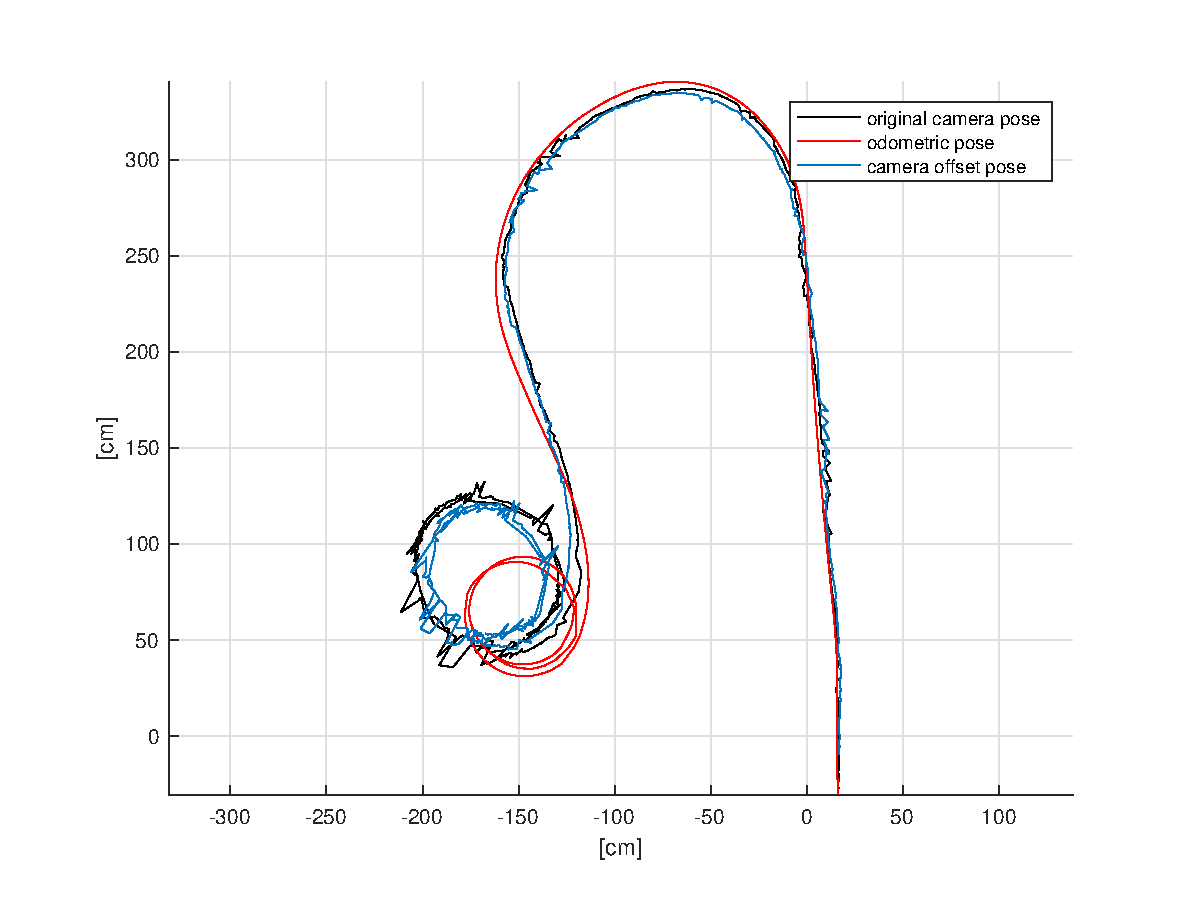
\includegraphics[width=0.5\textwidth]{recostropt_1}}
   \caption{Optimal odometric and camera position, dataset: 1}
   \label{fig:OptiOdo1}
\end{figure}

\begin{figure}[h]
   {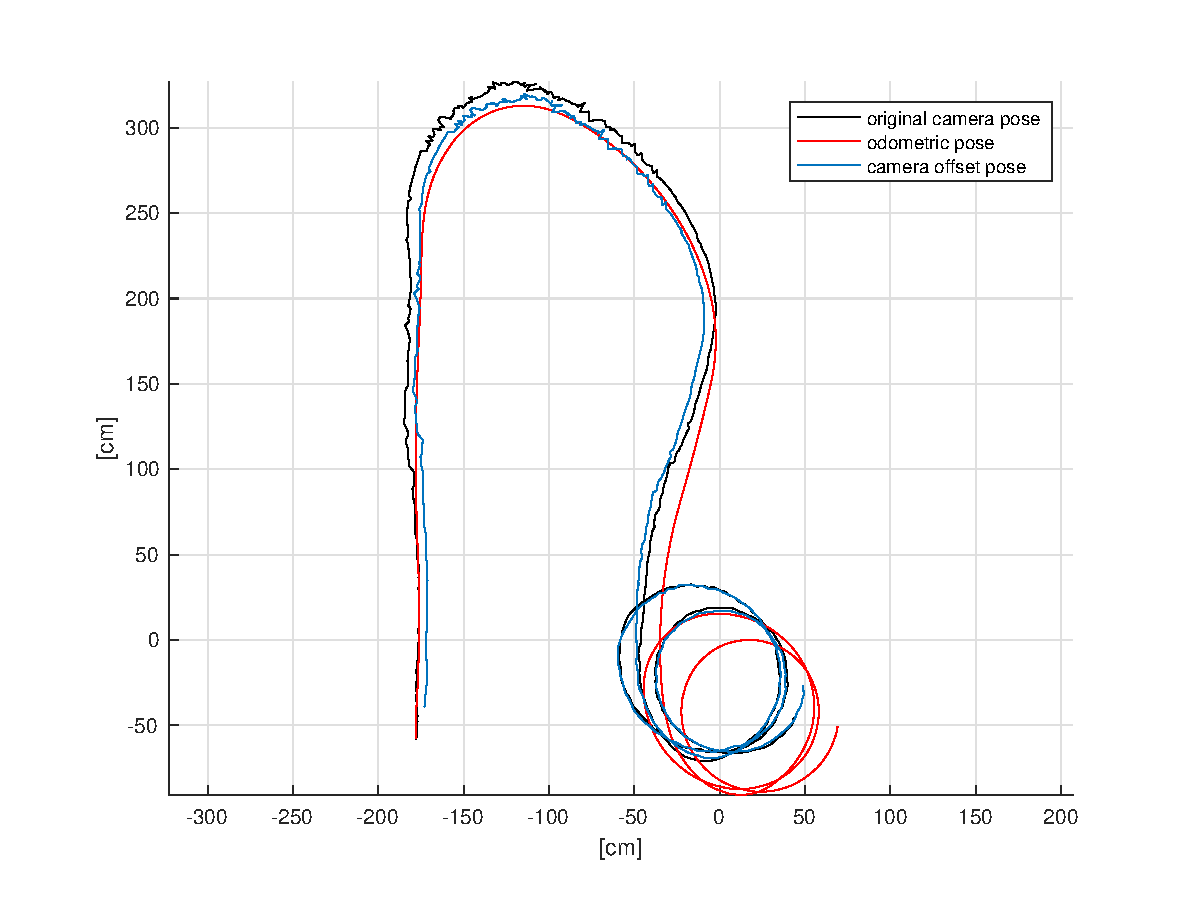
\includegraphics[width=0.5\textwidth]{recostropt_2}}
   \caption{Optimal odometric and camera position, dataset: 2}
   \label{fig:OptiOdo2}
\end{figure}

\begin{figure}[h]
   {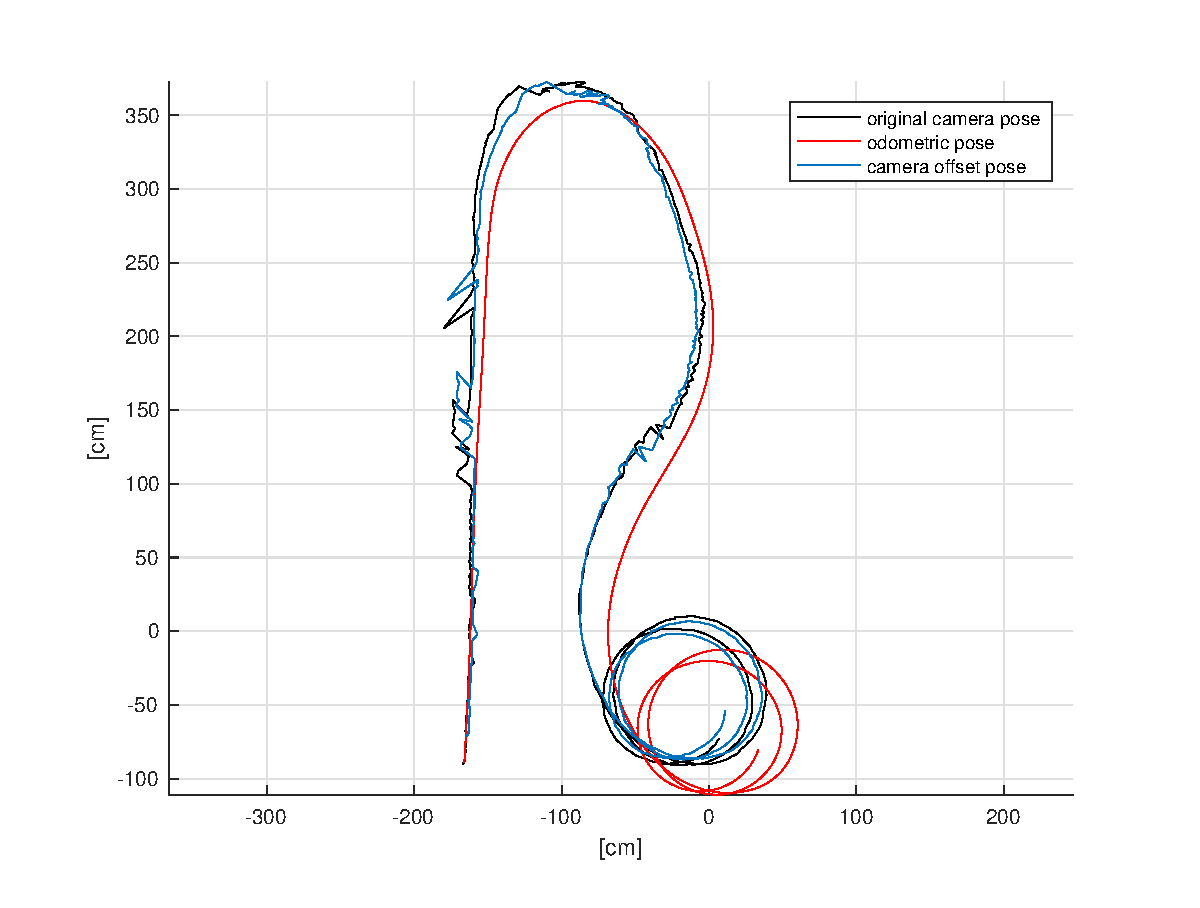
\includegraphics[width=0.5\textwidth]{recostropt_3}} 
   \caption{Optimal odometric and camera position, dataset: 3}
   \label{fig:OptiOdo3}
\end{figure}

\begin{figure}[h]
   {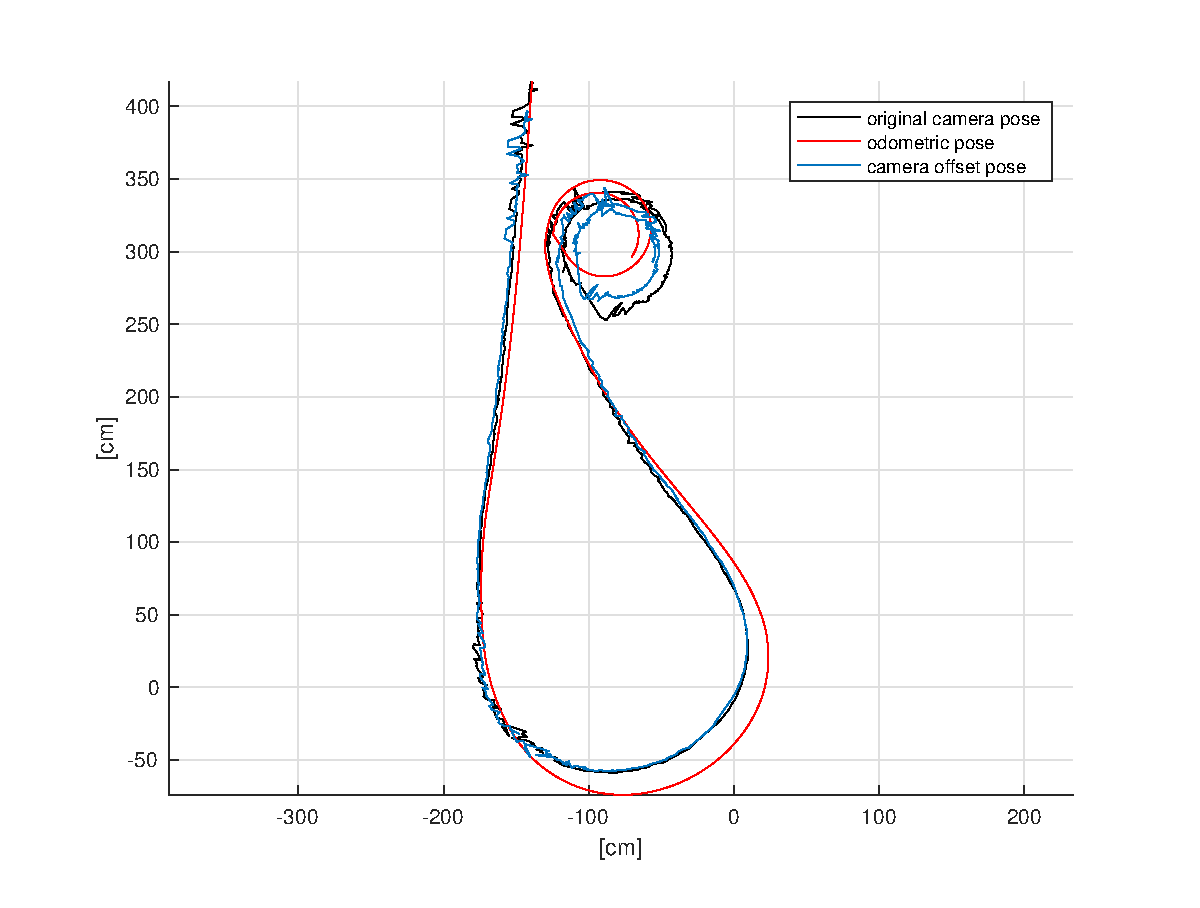
\includegraphics[width=0.5\textwidth]{recostropt_4}}
\caption{Optimal odometric and camera position, dataset: 4}
\label{fig:OptiOdo4}
\end{figure}
	\section{Results}
Using the scientific article by proposed method allows to obtain the values obtained in the table, it is observed that the distance between the robot's actual parameters and those estimates are introduced by the assumed model simplifications and errors.
In the first analysis, the method proposed, treats that the odometric center placed in mid's robot axle as well as in the model used, but does not take account that the camera's position may be not aligned with point previously analyzed.
Errors also depend on assumptions regarding the non-deformability of the wheels and the tire above keyed, any misalignments. The motion is achieved by considering a regular and uniform surface, and then ignoring bumps, obstacles, unevenness, etc.
Also recommend to use predetermined paths, possibly, whereas those in a straight line, with counterclockwise and clockwise rotations in order to minimize errors and to allow independent calibration of the parameters.

%----------------------------------------------------------------------------------------
%	Bibliography
%----------------------------------------------------------------------------------------
	
	\bibliographystyle{IEEEtran}
	\bibliography{bibliografy.bib}

%----------------------------------------------------------------------------------------
%	Programming Languages
%---------------------------------------------------------------------------------------- 
	\onecolumn
	\lstinputlisting[language=iPython,label=lang:codePython,caption=main.py]{/Users/francescoargentieri/Kinematics-Calibration-of-a-Differential-drive/Data/PythonScript/main.py}
	\lstinputlisting[language=iPython,label=lang:codePythonPd,caption=dataframe.py]{/Users/francescoargentieri/Kinematics-Calibration-of-a-Differential-drive/Data/PythonScript/dataframe.py}
	\newpage	
	\lstinputlisting[language=Matlab,label=lang:MatlabObjFunc,caption=ObjectiveFunction.m]{/Users/francescoargentieri/Kinematics-Calibration-of-a-Differential-drive/Optimization/gaerror.m}
\end{document}
